\documentclass[11pt,a4paper]{report}

% -- Geometry ------------------------------------------------------------------
\usepackage[a4paper, margin=1in, headheight=14pt]{geometry}

% -- Fonts & encoding ----------------------------------------------------------
\usepackage[T1]{fontenc}
\usepackage[utf8]{inputenc}
\usepackage{lmodern}

% -- Mathematics ---------------------------------------------------------------
\usepackage{amsmath, amssymb, amsthm}
\usepackage{bm}
\usepackage{mathtools}

% -- Graphics & colour ---------------------------------------------------------
\usepackage{graphicx}
\graphicspath{{figures/}}          % all figures live in figures/
\usepackage[dvipsnames, svgnames, x11names]{xcolor}
\usepackage{tikz}
\usetikzlibrary{arrows.meta, positioning, calc, shapes.geometric,
                decorations.markings, patterns}

% -- KIT colour palette  (MUST come before hyperref) ---------------------------
\definecolor{KITgreen}{HTML}{009682}
\definecolor{KITblue}{HTML}{4664AA}
\definecolor{navy}{HTML}{0D1B2A}
\definecolor{coral}{HTML}{D85A30}
\definecolor{boxbg}{HTML}{F0F6F6}
\definecolor{warnbg}{HTML}{FFF1ED}

% -- Tables --------------------------------------------------------------------
\usepackage{booktabs}
\usepackage{array}
\usepackage{multirow}

% -- Captions & floats ---------------------------------------------------------
\usepackage{caption}
\usepackage{subcaption}
\usepackage{float}

% -- Lists ---------------------------------------------------------------------
\usepackage{enumitem}

% -- Coloured boxes ------------------------------------------------------------
\usepackage[most]{tcolorbox}

% -- Headers & footers ---------------------------------------------------------
\usepackage{fancyhdr}
\pagestyle{fancy}
\fancyhf{}
\fancyhead[L]{\small\leftmark}
\fancyhead[R]{\small Ni/TiO$_2$ HMM Characterisation}
\fancyfoot[C]{\thepage}
\renewcommand{\headrulewidth}{0.4pt}

% -- Chapter title style -------------------------------------------------------
\usepackage{titlesec}
\titleformat{\chapter}[display]
  {\normalfont\huge\bfseries\color{KITgreen}}
  {\chaptertitlename\ \thechapter}{16pt}{\Huge}
\titlespacing*{\chapter}{0pt}{-20pt}{20pt}

% -- Bibliography  (MUST come before hyperref) ---------------------------------
\usepackage[numbers,sort&compress]{natbib}
\bibliographystyle{unsrtnat}

% -- Hyperlinks  (MUST come last among these packages) -------------------------
\usepackage[colorlinks=true, linkcolor=KITgreen, citecolor=KITgreen,
            urlcolor=KITblue, bookmarks=true]{hyperref}

% -- Custom boxes (colours already defined above) ------------------------------
\newtcolorbox{resultbox}{
  colback=boxbg, colframe=KITgreen, boxrule=0.6pt,
  arc=2pt, left=8pt, right=8pt, top=6pt, bottom=6pt,
  fonttitle=\bfseries, title={Result}}

\newtcolorbox{warnbox}{
  colback=warnbg, colframe=coral, boxrule=0.6pt,
  arc=2pt, left=8pt, right=8pt, top=6pt, bottom=6pt,
  fonttitle=\bfseries, title={Important}}

\newtcolorbox{derivbox}{
  colback=KITblue!5, colframe=KITblue, boxrule=0.6pt,
  arc=2pt, left=8pt, right=8pt, top=6pt, bottom=6pt,
  fonttitle=\bfseries, title={Derivation}}

% -- Global macros -------------------------------------------------------------
\newcommand{\ii}{\mathrm{i}}
\newcommand{\ee}{\mathrm{e}}
\renewcommand{\Re}{\operatorname{Re}}
\renewcommand{\Im}{\operatorname{Im}}
\newcommand{\eps}{\varepsilon}
\newcommand{\epar}{\eps_{\parallel}}
\newcommand{\eperp}{\eps_{\perp}}
\newcommand{\nt}{\tilde{n}}
\newcommand{\kt}{\tilde{k}}
\newcommand{\kzero}{k_0}
\newcommand{\kvec}{\bm{k}}
\newcommand{\Evec}{\bm{E}}
\newcommand{\Hvec}{\bm{H}}
\newcommand{\Dvec}{\bm{D}}
\newcommand{\Bvec}{\bm{B}}
\newcommand{\rp}{r_{\mathrm{p}}}
\newcommand{\rs}{r_{\mathrm{s}}}
\newcommand{\tp}{t_{\mathrm{p}}}
\newcommand{\ts}{t_{\mathrm{s}}}
\newcommand{\lam}{\lambda}

% =============================================================================
\begin{document}

% -- Title page ----------------------------------------------------------------
\begin{titlepage}
\centering
\vspace*{2.5cm}
{\color{KITgreen}\rule{\linewidth}{1.2pt}}\par
\vspace{0.6cm}
{\LARGE\bfseries Optical Characterisation of a Ni/TiO$_2$\par}
\vspace{0.3cm}
{\LARGE\bfseries Hyperbolic Metamaterial\par}
\vspace{0.3cm}
{\large From Maxwell's Equations to Isofrequency Contour Reconstruction\par}
\vspace{0.4cm}
{\color{KITgreen}\rule{\linewidth}{1.2pt}}\par
\vspace{1.4cm}
{\large\itshape
  Theory, effective-medium modelling, transfer matrix derivation,\\[4pt]
  ellipsometric inverse extraction, and IFC reconstruction\par}
\vfill
\begin{tabular}{rl}
  \textbf{Author}      & Mohammad Ashraful Haque \\[4pt]
  \textbf{Affiliation} & Master's Student, KSOP \\[2pt]
                       & Research Assistant, Institute of Nanotechnology, KIT \\[2pt]
                       & Research Assistant, Deeplight GmbH \\[6pt]
  \textbf{Supervisor}  & Prof.\ Dr.\ Maryna L.\ Meretska \\[2pt]
                       & Institute of Nanotechnology, KIT \\[6pt]
  \textbf{Date}        & \today
\end{tabular}
\vspace{2.0cm}
\end{titlepage}

% -- Abstract ------------------------------------------------------------------
\chapter*{Abstract}
\addcontentsline{toc}{chapter}{Abstract}
\noindent
This report provides a comprehensive, first-principles treatment of the optical
characterisation of a three-period [TiO$_2$/Ni]$\times$3 hyperbolic metamaterial
(HMM) deposited on a borosilicate glass (SiO$_2$) substrate. Starting from
Maxwell's equations, we derive the uniaxial electromagnetic dispersion relation,
effective-medium theory (EMT), and the complete transfer matrix method (TMM) for
anisotropic multilayer stacks, applied step by step to the FIB/TEM-measured
per-layer thicknesses of the fabricated sample. We document systematically why
angle-resolved reflectance and transmittance measurements are fundamentally
insufficient to recover the out-of-plane permittivity $\eperp$ at sub-wavelength
film thicknesses---a consequence of the evanescent suppression of the $E_z$ field
component across a \mbox{44\,nm} stack---and how spectroscopic ellipsometry resolves
this through phase-sensitive multi-angle inversion. The extracted permittivity
tensor $(\epar(\lambda),\,\eperp(\lambda))$ is used to reconstruct the
isofrequency contour (IFC) via the Jackson et al.\ (2024) lossy complex-wavevector
method. The central finding is that both $\Re(\epar)$ and $\Re(\eperp)$ remain
positive throughout $550$--$1000$\,nm, producing a closed elliptical IFC with no
hyperbolic transition in the measured spectral window.

\clearpage

% -- Table of contents ---------------------------------------------------------
\tableofcontents
\clearpage

% -- Chapters ------------------------------------------------------------------
% Chapter 1: Introduction and Motivation
% Status: STUB -- content to be written

\chapter{Introduction and Motivation}

\textit{This chapter is under preparation.}

% Chapter 2: Electromagnetic Theory of a Uniaxial Medium
% Status: STUB -- content to be written

\chapter{Electromagnetic Theory of a Uniaxial Medium}
\label{ch:em_theory}

\textit{This chapter is under preparation.}

% Effective Medium Theory for Ni/TiO$_2$
% Status: STUB -- content to be written

\chapter{Effective Medium Theory for Ni/TiO$_2$}
\label{ch:emt}

\textit{This chapter is under preparation.}

% =============================================================================
% Chapter 4: Sample and Measurements
% =============================================================================

\chapter{Sample and Measurements}
\label{ch:sample_measurements}

This chapter describes the physical sample studied in this report and the two
independent sets of optical measurements performed on it. The first measurement,
angle-resolved reflectance and transmittance, provided the initial characterisation
of the stack and revealed that the R/T data alone could not reconstruct the
isofrequency contour. The second measurement, spectroscopic ellipsometry, was
introduced specifically to address this limitation and forms the experimental
basis for the permittivity extraction in Chapter~\ref{ch:inverse_methodology}.

% -----------------------------------------------------------------------------
\section{The Sample: A Three-Period Ni/TiO\texorpdfstring{$_2$}{2} Multilayer}
% -----------------------------------------------------------------------------

The sample studied throughout this report is a six-layer alternating stack of
nickel and titanium dioxide deposited on a borosilicate glass substrate. The
deposition order, from the substrate upward, is
\begin{equation}
  \text{SiO}_2\;\text{(substrate)} \;\Big|\;
  \underbrace{\text{Ni} \;\Big|\; \text{TiO}_2}_{\times\,3} \;\Big|\;
  \text{air},
\end{equation}
so that Ni is deposited directly on the glass and TiO$_2$ faces the air. This
orientation means that, when measuring from the air side, the wave first
encounters TiO$_2$, which is optically smoother and more transmissive than a
Ni surface, before entering the first metallic layer.

\paragraph{Deposition method.}
The Ni layers were deposited by physical vapour deposition (PVD) under high
vacuum. The TiO$_2$ layers were grown by atomic layer deposition (ALD). The
combination of PVD for the metal and ALD for the dielectric is a common
approach for producing Ni/TiO$_2$ multilayers, since ALD produces conformal,
pinhole-free TiO$_2$ films with excellent thickness control even on rough
underlying surfaces.

\paragraph{Layer thicknesses.}
The individual layer thicknesses were measured by focused ion beam
cross-sectional transmission electron microscopy (FIB/TEM) on a cleaved cross
section of the sample. The method provides direct sub-nanometre resolution of
each individual layer. The measured thicknesses are listed in
Table~\ref{tab:ch1_thicknesses} in Chapter~\ref{ch:introduction} and are used
without modification in all subsequent modelling. The total stack thickness is
$44.3$\,nm and the Ni fill fraction is $\rho = 0.379$.

\paragraph{Substrate identification.}
A key step in the analysis was confirming the optical identity of the substrate.
Two candidate substrates were tested in the transfer matrix forward model:
silicon (Si, using the constants of Green (2008)~\cite{green2008}) and fused
silica (SiO$_2$, using the Malitson Sellmeier formula~\cite{malitson}). The
root-mean-square residual between the ellipsometric model and the measured NCS
data was approximately $0.001$ for the SiO$_2$ substrate and approximately
$0.012$ for the Si substrate. The borosilicate glass substrate is therefore
confirmed as optically equivalent to fused silica in the spectral range of the
measurement. All subsequent calculations use the Malitson SiO$_2$ dispersion.

% -----------------------------------------------------------------------------
\section{Measurement 1: Angle-Resolved Reflectance and Transmittance}
% -----------------------------------------------------------------------------

The first set of measurements consisted of spectrally resolved reflectance
$R(\lambda)$ and transmittance $T(\lambda)$ acquired at near-normal incidence
over the wavelength range $400$ to $1000$\,nm. The absorbed fraction
$A(\lambda) = 1 - R(\lambda) - T(\lambda)$ was computed directly from the
measured $R$ and $T$.

Figure~\ref{fig:ch4_setup_rt} shows the measurement geometry. A collimated
white-light beam is directed at the sample surface, and the intensities of the
specularly reflected and directly transmitted beams are detected simultaneously.
The reflectance $R$ is measured as the ratio of the reflected intensity to a
reference intensity recorded without the sample, and the transmittance $T$
is measured as the ratio of the transmitted intensity to the same reference.

\begin{figure}[h]
\centering
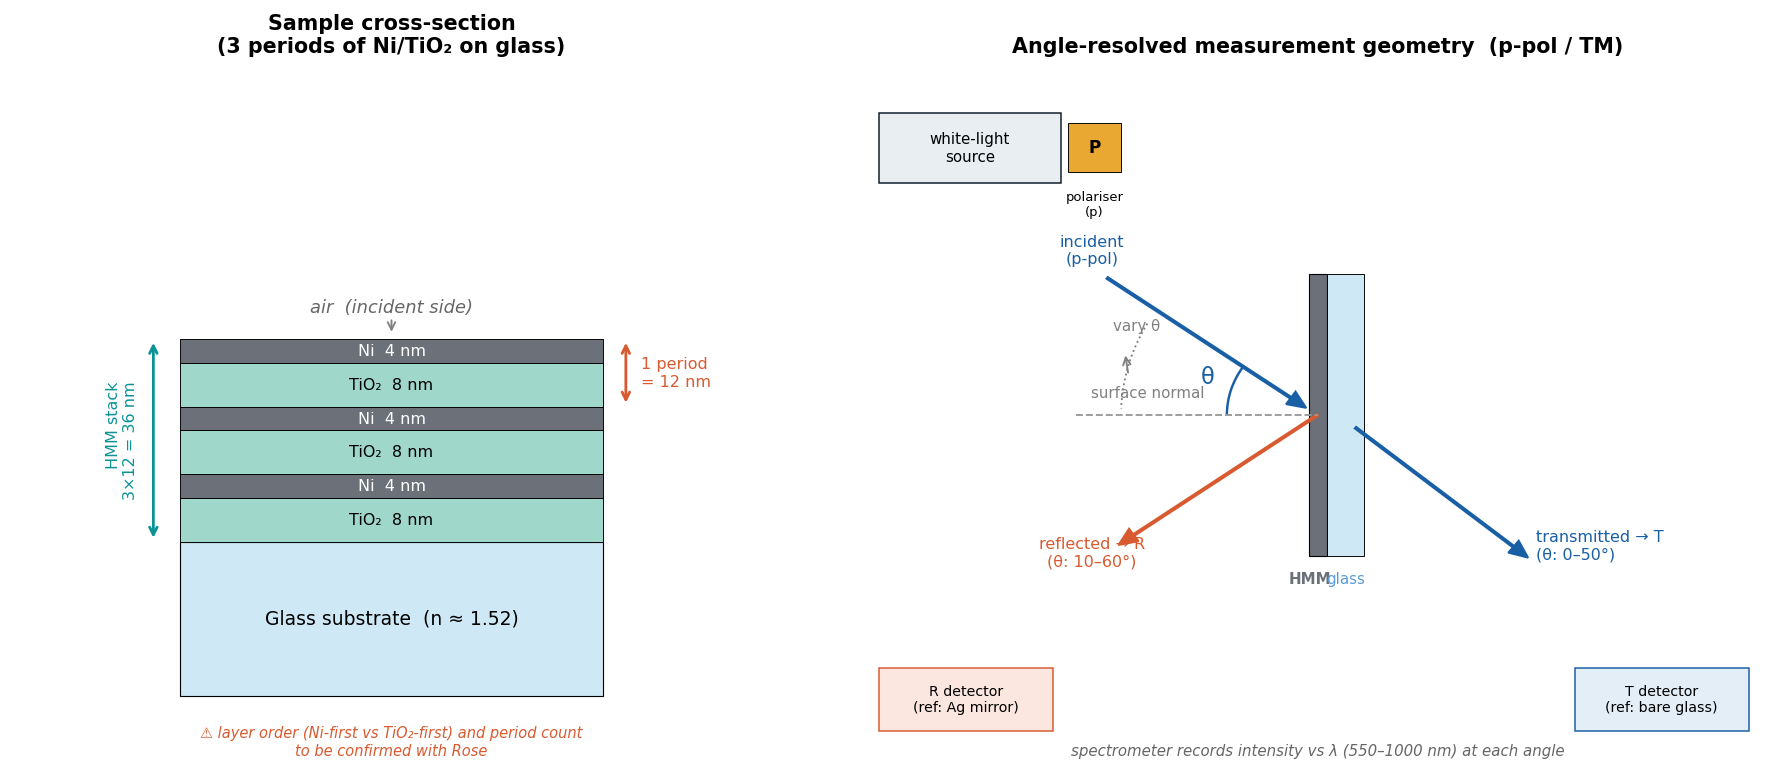
\includegraphics[width=0.70\textwidth]{figures/NiTiO2_setup_schematic.png}
\caption{Experimental setup for the angle-resolved reflectance and
  transmittance measurement. A collimated white-light beam is incident on the
  Ni/TiO$_2$ multilayer sample on a SiO$_2$ substrate. The reflected and
  transmitted intensities are recorded as a function of wavelength and used
  to compute $R(\lambda)$, $T(\lambda)$, and $A(\lambda) = 1 - R - T$.
  This measurement provided the initial optical characterisation of the stack
  but, as discussed in Chapter~\ref{ch:why_rt_failed}, was insufficient to
  recover the out-of-plane permittivity $\eperp$ and therefore could not
  reconstruct the isofrequency contour.}
\label{fig:ch4_setup_rt}
\end{figure}

Figure~\ref{fig:ch4_data_summary} shows the measured $R$, $T$, and $A$ spectra.

\begin{figure}[h]
\centering
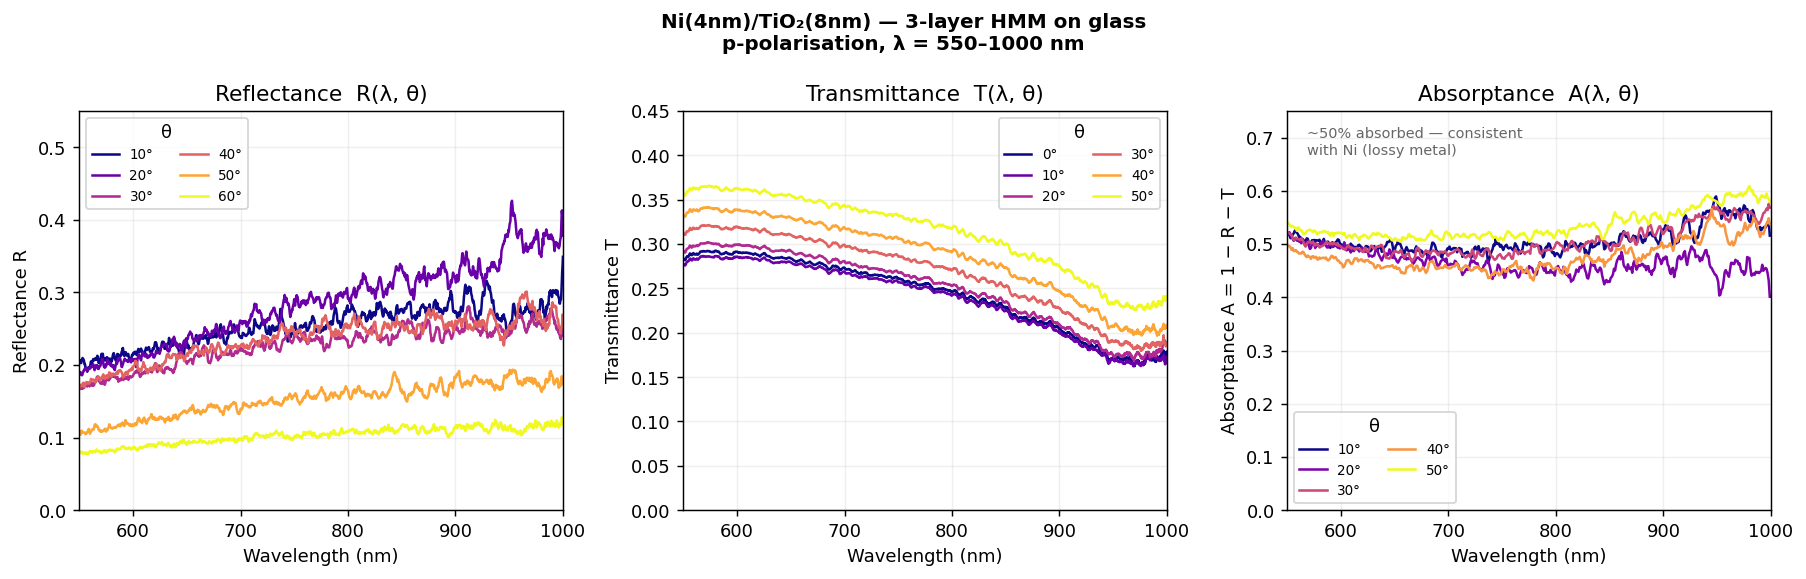
\includegraphics[width=0.85\textwidth]{figures/NiTiO2_data_summary.png}
\caption{Measured reflectance $R(\lambda)$, transmittance $T(\lambda)$, and
  absorptance $A(\lambda) = 1 - R - T$ of the [TiO$_2$/Ni]$\times$3
  multilayer on SiO$_2$ over the wavelength range $400$ to $1000$\,nm.
  The stack is strongly absorbing throughout, with $A > 0.3$ at all
  wavelengths. No Fabry-P\'{e}rot interference fringes are visible, consistent
  with the sub-wavelength total thickness ($44.3$\,nm) discussed in
  Chapter~\ref{ch:em_theory}. The smooth, featureless spectra confirm that
  the stack is in the effective medium regime.}
\label{fig:ch4_data_summary}
\end{figure}

Several features of the spectra are noteworthy.

\paragraph{Strong absorption throughout.}
The absorptance exceeds $0.3$ at all wavelengths across the measurement window.
This reflects the dominant contribution of the Ni layers, which absorb strongly
at visible frequencies. A purely dielectric stack of the same total thickness
would transmit more than $90\%$ of the incident light. The large absorptance
confirms that the Ni layers are optically active and that the in-plane
permittivity $\epar$ carries a large imaginary part, as discussed in
Chapter~\ref{ch:emt}.

\paragraph{No Fabry-P\'{e}rot fringes.}
The $R$, $T$, and $A$ spectra are smooth and featureless across the entire
measurement window. No oscillatory fringes are visible. This is expected for
a stack whose total thickness ($44.3$\,nm) is far below the wavelength of
the first fringe, as shown in Chapter~\ref{ch:em_theory}. The absence of
fringes confirms that no direct Fabry-P\'{e}rot wavevector reconstruction
is possible from this data.

\paragraph{What R/T cannot tell us.}
The reflectance and transmittance data are real, non-negative intensity
measurements. They cannot reveal the phase of the reflected or transmitted
fields, and, as we demonstrate in Chapter~\ref{ch:why_rt_failed}, the
sensitivity of $R$ and $T$ to the out-of-plane permittivity $\eperp$ is
vanishingly small for a $44.3$\,nm film. The R/T data alone are therefore
insufficient to extract the full permittivity tensor or to reconstruct the
isofrequency contour.

% -----------------------------------------------------------------------------
\section{Measurement 2: Spectroscopic Ellipsometry}
% -----------------------------------------------------------------------------

Spectroscopic ellipsometry was performed using a J.A.\ Woollam M-2000
variable angle spectroscopic ellipsometer (VASE) in the rotating compensator
configuration. This instrument measures the change in the polarisation state
of light upon specular reflection from a surface and has a spectral range of
approximately $245$ to $1700$\,nm.

\subsection{The Ellipsometric Observables: \texorpdfstring{$\Psi$, $\Delta$,
  and the NCS Parameters}{Psi, Delta, and the NCS Parameters}}

When a linearly polarised plane wave reflects from a surface, the amplitudes
and phases of the $p$- and $s$-polarised components change independently.
The complex reflection coefficients $\rp$ and $\rs$ define the ellipsometric
ratio
\begin{equation}
  \rho_\text{ell} \equiv \frac{\rp}{\rs} = \tan\Psi\,\ee^{\ii\Delta},
  \label{eq:ch4_ellipsometric_ratio}
\end{equation}
where $\Psi \in [0^\circ, 90^\circ]$ is the amplitude ratio angle and
$\Delta \in [0^\circ, 360^\circ]$ is the phase difference between the
$p$- and $s$-polarised reflections. Together, $\Psi$ and $\Delta$ fully
characterise the polarisation change upon reflection.

In practice, the M-2000 instrument does not report $\Psi$ and $\Delta$
directly. Instead, it exports data in the Stokes-like NCS representation:
\begin{align}
  N &= \cos 2\Psi, \label{eq:ch4_N} \\
  C &= \sin 2\Psi\,\cos\Delta, \label{eq:ch4_C} \\
  S &= \sin 2\Psi\,\sin\Delta. \label{eq:ch4_S}
\end{align}
The NCS parameters are preferred over $\Psi$ and $\Delta$ directly because they
are bounded ($N, C, S \in [-1, 1]$), linearly related to the Stokes parameters
of the reflected beam, and free from the $\pi$-periodicity ambiguity that
affects $\Psi$. They are also the natural output of the rotating compensator
measurement principle used in the M-2000.

\begin{warnbox}
\textbf{CompleteEASE sign convention.} The M-2000 instrument and its
companion software, CompleteEASE, use a sign convention for $\Delta$ that is
opposite to the convention used in the standard \texttt{tmm} Python package
and in many textbooks. Specifically, the CompleteEASE convention defines the
phase difference as $\Delta_\text{CE} = -\Delta_\text{standard}$, which means
$S_\text{CE} = -S_\text{standard}$ while $N$ and $C$ are unaffected. Failing
to account for this sign difference produces a systematic error in $\Delta$ of
$180^\circ$ at all angles, which completely invalidates the permittivity
extraction. All modelling in this report uses the CompleteEASE convention
by negating $S$ (equivalently, negating $C$ and $S$) in the forward model
before comparing with the measured data.
\end{warnbox}

\subsection{Instrument Configuration and Measurement Protocol}

The M-2000 operates in the PCSA configuration: Polariser, Compensator (rotating),
Sample, Analyser. Figure~\ref{fig:ch4_ellipsometry_setup} illustrates this
arrangement. The broadband light source produces a collimated beam that passes
through a fixed linear polariser and then through a continuously rotating
waveplate (the compensator). The resulting beam, which has a time-varying
elliptical polarisation, reflects from the sample surface and passes through a
fixed analyser before being dispersed onto a CCD detector array.

\begin{figure}[h]
\centering
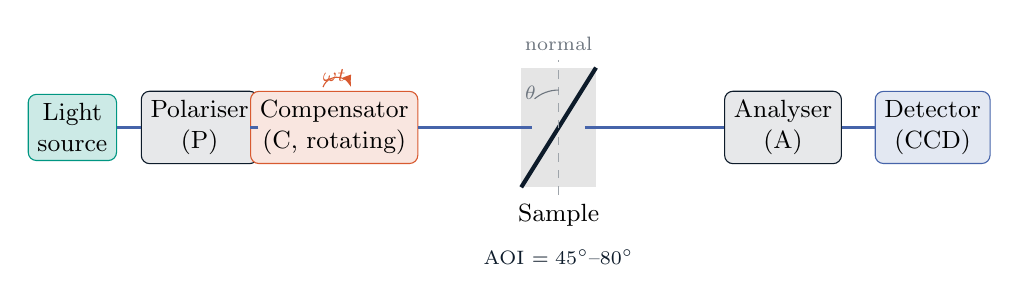
\begin{tikzpicture}[scale=0.95,
  comp/.style={draw=navy, fill=navy!10, rounded corners=3pt,
               minimum width=1.1cm, minimum height=0.7cm, font=\small,
               align=center},
  arr/.style={-{Latex[length=2.5mm]}, thick, color=KITblue},
  beam/.style={very thick, color=KITblue},
  ifc/.style={thick, color=navy},
  lbl/.style={font=\small, align=center}
]

% Light source
\node[comp, fill=KITgreen!20, draw=KITgreen] (src) at (-6.5, 0)
  {Light\\source};

% Polariser
\node[comp] (pol) at (-4.8, 0) {Polariser\\(P)};

% Compensator (rotating)
\node[comp, fill=coral!15, draw=coral] (comp) at (-3.0, 0)
  {Compensator\\(C, rotating)};

% Sample surface (tilted)
\begin{scope}[shift={(0, 0)}]
  \fill[gray!20] (-0.5,-0.8) -- (0.5,-0.8) -- (0.5, 0.8) -- (-0.5, 0.8) -- cycle;
  \draw[ifc, line width=1.5pt] (-0.5,-0.8) -- (0.5, 0.8);
  \node[below, font=\small] at (0,-0.9) {Sample};
\end{scope}

% Analyser
\node[comp] (ana) at (3.0, 0) {Analyser\\(A)};

% Detector
\node[comp, fill=KITblue!15, draw=KITblue] (det) at (5.0, 0)
  {Detector\\(CCD)};

% Incident beam (from source to sample)
\draw[beam] (src.east) -- (pol.west);
\draw[beam] (pol.east) -- (comp.west);
\draw[beam] (comp.east) -- (-0.35, 0);

% Reflected beam (from sample to analyser)
\draw[beam] (0.35, 0) -- (ana.west);
\draw[beam] (ana.east) -- (det.west);

% Angle of incidence label
\draw[dashed, color=navy!40] (0,-0.9) -- (0, 0.9)
  node[above, font=\scriptsize, color=navy!60] {normal};
\draw[color=navy!60] (0, 0.5) arc (90:130:0.5)
  node[midway, left, font=\scriptsize] {$\theta$};

% Rotating arrow on compensator
\draw[-{Latex[length=1.5mm]}, coral, thin]
  ($(comp.north) + (-0.15, 0.05)$) arc (160:20:0.2);
\node[above, font=\scriptsize, color=coral] at (comp.north) {$\omega t$};

% AOI label
\node[below, font=\scriptsize, color=navy] at (0,-1.5)
  {AOI $= 45^\circ$--$80^\circ$};

\end{tikzpicture}
\caption{PCSA configuration of the J.A.\ Woollam M-2000 spectroscopic
  ellipsometer. A broadband beam passes through a fixed polariser and a
  rotating compensator (waveplate, rotating at angular frequency $\omega$),
  reflects from the sample at a chosen angle of incidence $\theta$, and is
  analysed by a fixed analyser before reaching the CCD detector. The rotating
  compensator modulates the polarisation state of the incident beam
  periodically, and the detector records the resulting intensity variation.
  Fourier analysis of this variation yields $\Psi(\lambda)$ and
  $\Delta(\lambda)$, or equivalently $N$, $C$, $S$, at every wavelength
  simultaneously.}
\label{fig:ch4_ellipsometry_setup}
\end{figure}

Data were collected at \textbf{eight angles of incidence}: $45^\circ$,
$50^\circ$, $55^\circ$, $60^\circ$, $65^\circ$, $70^\circ$, $75^\circ$,
and $80^\circ$, measured from the surface normal. At each angle, the three
NCS spectra were acquired simultaneously over the spectral range $450$ to
$1000$\,nm at a wavelength resolution of approximately $1.6$\,nm, yielding
a total dataset of $24$ spectra ($3 \times 8$ AOIs). The large number of
angles is essential for constraining the out-of-plane permittivity $\eperp$:
each additional angle provides an independent measurement that further
narrows the uncertainty on $\eperp$, as discussed in
Chapter~\ref{ch:why_rt_failed}.

\subsection{Why Eight Angles and Why Up to \texorpdfstring{$80^\circ$}{80 degrees}}

The choice of eight angles spanning $45^\circ$ to $80^\circ$ deserves
explanation. At angles below $45^\circ$, the difference between the
$p$- and $s$-polarised Fresnel coefficients becomes small, reducing the
ellipsometric sensitivity. At angles above $80^\circ$, the beam footprint
on the sample becomes very elongated, introducing beam-edge artefacts and
averaging over a larger sample area with potential thickness inhomogeneities.

The upper end of the range, $75^\circ$ to $80^\circ$, is particularly
important for this sample. The pseudo-Brewster angle of the stack, the
angle at which $|r_p|$ reaches a minimum and $\Delta$ changes rapidly,
occurs near $75^\circ$ at most wavelengths. This rapid variation of $\Delta$
near the pseudo-Brewster angle is the most sensitive region for detecting
$\eperp$, as we show quantitatively in Chapter~\ref{ch:why_rt_failed}. The
measurement at $75^\circ$ and $80^\circ$ is therefore not redundant with
the lower angles: it provides qualitatively different sensitivity to the
out-of-plane response.

% -----------------------------------------------------------------------------
\section{Summary of the Experimental Dataset}
% -----------------------------------------------------------------------------

Table~\ref{tab:ch4_dataset} summarises the two experimental datasets used in
this report.

\begin{table}[h]
\centering
\caption{Summary of the two optical datasets used for characterisation of the
  [TiO$_2$/Ni]$\times$3 multilayer. All measurements were performed at room
  temperature on the same sample.}
\label{tab:ch4_dataset}
\begin{tabular}{lll}
\toprule
Property & R/T measurement & Ellipsometry \\
\midrule
Instrument          & Custom white-light setup  & J.A.\ Woollam M-2000 VASE \\
Configuration       & Near-normal incidence     & PCSA rotating compensator \\
Spectral range      & $400$--$1000$\,nm         & $450$--$1000$\,nm \\
Angles of incidence & Near-normal ($\approx 0^\circ$) & $45^\circ$, $50^\circ$, $55^\circ$,
                                                           $60^\circ$, $65^\circ$, $70^\circ$,
                                                           $75^\circ$, $80^\circ$ \\
Observables         & $R(\lambda)$, $T(\lambda)$ & $N(\lambda,\theta)$, $C(\lambda,\theta)$,
                                                   $S(\lambda,\theta)$ \\
Number of spectra   & 2                         & 24 ($3\times 8$ AOIs) \\
Sensitive to        & $\epar$ (primarily)       & Both $\epar$ and $\eperp$ \\
Can reconstruct IFC?& No (see Ch.~\ref{ch:why_rt_failed}) & Yes (see Ch.~\ref{ch:results}) \\
\bottomrule
\end{tabular}
\end{table}

The contrast between the two datasets motivates the structure of the rest of
this report. Chapters~\ref{ch:tmm_derivation} and~\ref{ch:forward_validation}
develop and validate the forward model for both datasets.
Chapter~\ref{ch:why_rt_failed} demonstrates rigorously why the R/T data cannot
recover $\eperp$ and why the ellipsometric phase data can.
Chapters~\ref{ch:inverse_methodology} and~\ref{ch:results} then perform the
ellipsometric extraction and present the final reconstructed IFC.

\begin{resultbox}
\textbf{Summary of Chapter~\ref{ch:sample_measurements}.} The sample is a
[TiO$_2$/Ni]$\times$3 multilayer with FIB/TEM-measured per-layer thicknesses
summing to $44.3$\,nm ($\rho = 0.379$) on a SiO$_2$ substrate confirmed by
ellipsometric residual comparison. Two optical measurements were performed:
angle-resolved R/T (which showed strong absorption and no Fabry-P\'{e}rot
fringes but could not recover $\eperp$) and spectroscopic ellipsometry on a
J.A.\ Woollam M-2000 at eight angles of incidence from $45^\circ$ to
$80^\circ$, yielding $N$, $C$, $S$ spectra in the CompleteEASE sign
convention. The ellipsometric data at large angles, in particular near the
pseudo-Brewster angle at $75^\circ$, provide the sensitivity to $\eperp$
that the R/T data lacked.
\end{resultbox}

% Chapter 5: Transfer Matrix Method -- Step-by-Step Derivation
% Status: STUB -- content to be written

\chapter{Transfer Matrix Method: Step-by-Step Derivation}
\label{ch:tmm_derivation}

\textit{This chapter is under preparation.}

% Chapter 6: Forward Model Validation
% Status: STUB -- content to be written

\chapter{Forward Model Validation}
\label{ch:forward_validation}

\textit{This chapter is under preparation.}

% Chapter 7: Why R/T Failed and Why Ellipsometry Was Needed
% Status: STUB -- content to be written

\chapter{Why R/T Failed and Why Ellipsometry Was Needed}
\label{ch:why_rt_failed}

\textit{This chapter is under preparation.}

% Chapter 8: Inverse Extraction Methodology
% Status: STUB -- content to be written

\chapter{Inverse Extraction Methodology}
\label{ch:inverse_methodology}

\textit{This chapter is under preparation.}

% Chapter 9: Results and Physical Interpretation -- STUB
\chapter{Results and Physical Interpretation}
\textit{This chapter is under preparation.}

% Chapter 10: Limitations and Next Steps -- STUB
\chapter{Limitations and Next Steps}
\textit{This chapter is under preparation.}


% -- Bibliography --------------------------------------------------------------
\bibliography{references}

\end{document}
